\documentclass[aspectratio=169, 14pt]{beamer}
\usepackage[utf8]{inputenc}
\usepackage{xeCJK}
\usepackage{graphicx}
\usepackage{transparent}
\usepackage[ruled, lined, linesnumbered, commentsnumbered]{algorithm2e}
\usepackage{pgfplots}
\usepackage{tikz}
\usetikzlibrary{matrix,backgrounds}
\usetikzlibrary{arrows}
\usetikzlibrary {arrows.meta}
\usetikzlibrary{calc,shadows.blur,fit,positioning}
\usetikzlibrary {shapes.multipart}
\usetikzlibrary{chains}
\usetikzlibrary{er}
\usepackage{minted}
\usepackage{fontawesome5}
\usepackage{booktabs}
\usepackage{caption}
\usepackage{hyperref}
\hypersetup{
    colorlinks=true,
    linkcolor=blue,
    filecolor=magenta,      
    urlcolor=cyan,
    }
\urlstyle{same}
\usetheme{metropolis}
\metroset{block=fill}
\usecolortheme{default}
\definecolor{darkmidnightblue}{rgb}{0.0, 0.2, 0.4}
\definecolor{LightGray}{gray}{0.9}

\usepackage[normalem]{ulem}

%------------------------------------------------------------
%This block of code defines the information to appear in the
%Title page
\title[Database Principles and Applications] %optional
{数据库原理与应用}

\subtitle{ER模型}

\author[CHEN Zhongpu] % (optional)
{CHEN Zhongpu}

\institute[] % (optional)
{
  School of Computing and Artificial Intelligence \\
  \href{mailto:zpchen@swufe.edu.cn}{zpchen@swufe.edu.cn}
}

\date[] % (optional)
{SWUFE, Spring \the\year{}}

%End of title page configuration block
%------------------------------------------------------------


%------------------------------------------------------------
%The next block of commands puts the table of contents at the 
%beginning of each section and highlights the current section:

% \AtBeginSection[]
% {
%   \begin{frame}
%     \frametitle{Table of Contents}
%     \tableofcontents[currentsection]
%   \end{frame}
% }
%------------------------------------------------------------


\begin{document}

%The next statement creates the title page.
\frame{\titlepage}

%---------------------------------------------------------
%This block of code is for the table of contents after
%the title page
% \begin{frame}
% \frametitle{Table of Contents}
% \tableofcontents
% \end{frame}
%--------------------------------------------------------
\begin{frame}
    \frametitle{复习}
    \begin{center}
        \LARGE {\faIcon{database}}
    \end{center}
    \begin{enumerate}
        \item 如何使用数据库 (SQL)
        \item \alert{如何设计数据库}
        \item 如何实现数据库
    \end{enumerate}

\end{frame}

{
    % \usebackgroundtemplate{\transparent{0.3}{\begin{picture}
    %     
\includegraphics[height=0.7\paperheight]{cover}
    % \end{picture}    
    % }}
\usebackgroundtemplate{
  \tikz[overlay,remember picture] 
  \node[opacity=0.3, at=(current page.south east),anchor=south east, yshift=2cm,xshift=4cm] {
    
\includegraphics[height=0.6\paperheight]{cover}};
}
    \begin{frame}
        \section{\textcolor{darkmidnightblue}{1. 数据库设计概览}}
        如何将「需求」变成最终设计?
    \end{frame}
}

\begin{frame}
    \frametitle{1.1 设计阶段}
    对小型应用,一个数据库的设计者一般可以直接决定要构建的关系、关系的属性及其上的约束。

    但现实中的应该一般非常复杂,通常没有一个人能够理解应用的全部需求,所以为了沟通需求,应该将用户的需求\alert{分阶段}地用某种\alert{高级别}的方式表示出来,最后再将需求转化为\alert{较低级别}的设计。
\end{frame}

\begin{frame}[fragile]
    \begin{tikzpicture}[>=stealth,
        node distance = 3mm and 3mm,
          start chain = A going below right,
    every node/.style = {draw, text width=24mm, minimum height=12mm, align=center,
                         inner sep=1mm, fill=white, drop shadow={fill=black},  on chain=A},
                            ]
    \node (nreq) {需求分析}; % A-1
    \node {概念设计};
    \node {逻辑设计};
    \node {物理设计};
    %
    \foreach \i [count=\j] in {2,...,4}
    {
    %   \draw[->, thick] (A-\i) -| (A-\j);
      \draw[->, thick] (A-\j) -| (A-\i);
    }
    \end{tikzpicture}

    \begin{tikzpicture}
        \node[fill=blue!30,blur shadow={shadow xshift=-0.5ex},
        text width=16em,anchor=south west,rounded corners]
        {参考课本 p. 208:图7.2。};
    \end{tikzpicture}

\end{frame}

\begin{frame}[fragile]
    \frametitle{1.2 关于需求}

\includegraphics[width=.8\textwidth]{week10/hair1}

\pause
\begin{columns}
    \column{.4\textwidth}
    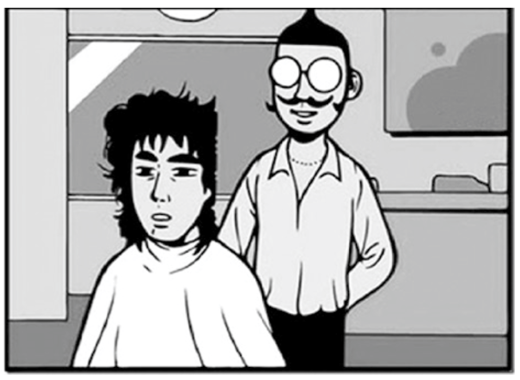
\includegraphics[width=.9\textwidth]{week10/hair2}
    \column{.6\textwidth}
    \begin{tikzpicture}
        \node[fill=yellow,blur shadow={shadow xshift=-0.5ex},
        text width=16em,anchor=south west,rounded corners]
        {理解用户的需求并不简单,并且可能用户也不知道自己的需求。};
    \end{tikzpicture}
\end{columns}

\end{frame}

% \begin{frame}
%     \frametitle{思考}
%
% \begin{columns}
%     \column{.5\textwidth}
%     数据库设计并运行后,修改 \rule{1cm}{0.15mm} 相对比较简单。
%
% \begin{itemize}
%     \item 逻辑模式
%     \item 物理模式
% \end{itemize}
%     \column{.5\textwidth}
%     \begin{tikzpicture}[
%         node distance=2cm,
%         title/.style={font=\color{black!50}\ttfamily, fill=orange!30,},
%         typetag/.style={rectangle, draw=black!50, font=\ttfamily, anchor=west}
%       ]
%         \node (decomp) [title] { \normalsize 视图层 (view level)};
%
%         \node (di) [below=of decomp.west, typetag, yshift=0.5cm] { view 1 };
%         \node (dr) [right=of di.west, typetag] { view 2 };
%         \node (dots) [right=of dr.west] {...};
%         \node (dnc) [right=of dots.west, typetag, xshift=-1cm] { view n };
%
%         \node [draw=black!50,  fit={(decomp) (di) (dr) (dots) (dnc)}] (view){};
%
%         \node[draw=black!50, below=of view, yshift=1cm,title](logical){逻辑层 (logical level)};
%
%         \node[draw=black!50, below=of logical, yshift=1cm,title](physical){物理层 (physical level)}; 
%
%         \draw[-, thick] (view) -- (logical);
%         \draw[-, thick] (logical) -- (physical);
%
%       \end{tikzpicture}
% \end{columns}
%
% \end{frame}


\begin{frame}
    \section{\textcolor{darkmidnightblue}{2. E-R模型}}
    实体(entity)-联系(relationship)模型在将现实世界的需求映射到概念模式上非常有用。
\end{frame}

\begin{frame}
    \frametitle{历史}
\begin{columns}
    \column{.3\textwidth}
    \begin{figure}
        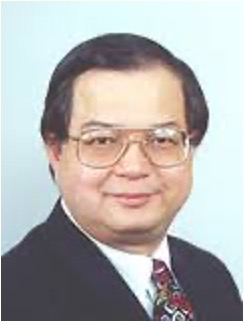
\includegraphics[width=\textwidth]{week10/chen}
        \caption*{Peter Pin-Shan Chen
        \\ 陳品山}
    \end{figure}
    \column{.69\textwidth}
    In software engineering, an ER model is commonly formed to represent things a business needs to remember in order to perform business processes. Consequently, the ER model becomes an abstract data model, that defines a data or information structure which can be implemented in a database, typically a relational database. 
\end{columns}

\end{frame}

\begin{frame}[fragile]
    \frametitle{2.1 实体与实体集}
与关系模式类似,实体(entity)通过一组属性表示。

\begin{exampleblock}{实体与实体集}
实体是现实世界中可区别所有其他对象的一个“事物”或“对象”。实体集(entity set)是相同类型的一个实体集合。    
\end{exampleblock}

\begin{columns}
    \column{.5\textwidth}
    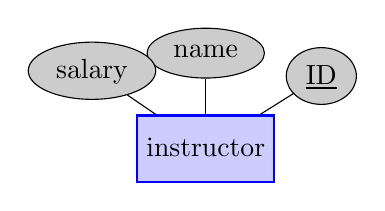
\begin{tikzpicture}[every pin edge/.style=draw, text depth=1pt,
        every attribute/.style={fill=black!20,draw=black},
        every entity/.style={fill=blue!20,draw=blue,thick},]
        \node[entity,pin={[attribute]30:\underline{ID}},pin={[attribute]90:name}, pin={[attribute]140:salary}] {instructor};
    \end{tikzpicture}
    \column{.5\textwidth}
    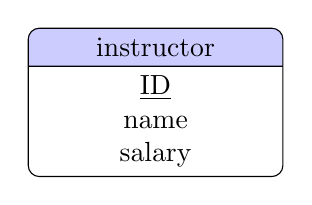
\begin{tikzpicture}[
        comment/.style={rectangle, draw=black, rounded corners,
        text centered, anchor=north, text=black, text width=3cm}, every second node part/.style={fill=white}]
        \node [comment, rectangle split, rectangle split parts=2, rectangle split part fill={blue!20,white}]
        {
            instructor
            \nodepart{second} \underline{ID} \\ name \\ salary
        };
    \end{tikzpicture}
\end{columns}

\end{frame}

\begin{frame}[fragile]
    \frametitle{2.2 联系与联系集}
\begin{exampleblock}{联系与联系集}
    联系(\texttt{relationship})是指多个实体间的相互关联。联系集(\texttt{relationship set})是相同类型联系的集合。
\end{exampleblock}


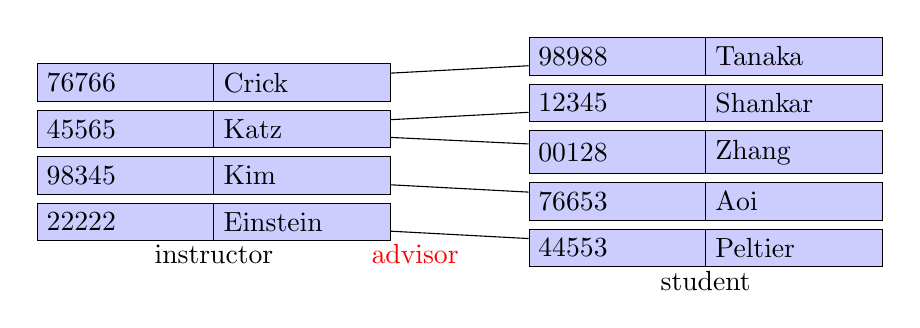
\begin{tikzpicture}
    \matrix (instructor)[row sep=.1cm, every node/.style={draw, fill=blue!20, rectangle split, rectangle split parts=2,rectangle split horizontal, text width=2cm,}]
    {
      \node (crick) {76766 \nodepart{two} Crick}; \\
      \node (katz) {45565 \nodepart{two} Katz}; \\
      \node (kim) {98345 \nodepart{two} Kim}; \\
      \node (ein) {22222 \nodepart{two} Einstein}; \\
    };
    \node (tinstructor)[below=of instructor, yshift=1.2cm] {instructor};

    \matrix (student)[right=of instructor, xshift=0.5cm, row sep=.1cm, every node/.style={draw, fill=blue!20, rectangle split, rectangle split parts=2,rectangle split horizontal, text width=2cm,}] {
        \node (tanaka) {98988 \nodepart{two} Tanaka}; \\
        \node (shankar) {12345 \nodepart{two} Shankar}; \\
        \node (zhang) {00128 \nodepart{two} Zhang}; \\
        \node (aoi) {76653 \nodepart{two} Aoi}; \\
        \node (pel) {44553 \nodepart{two} Peltier}; \\
    };
    \node[below=of student, yshift=1.2cm] {student};

    \draw (crick) -- (tanaka);
    \draw (katz) -- (shankar);
    \draw (katz) -- (zhang);
    \draw (kim) -- (aoi);
    \draw (ein) -- (pel);
    \node [right=of tinstructor, red] {advisor};
  \end{tikzpicture}

\end{frame}

\begin{frame}[fragile]
    \frametitle{E-R图}
    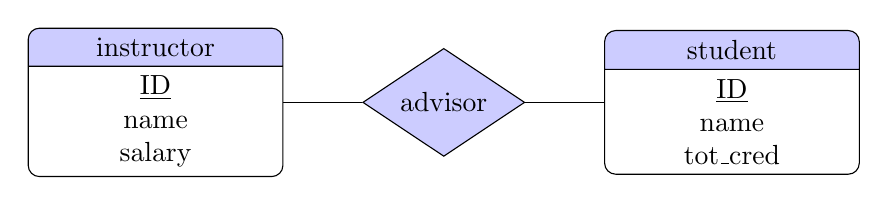
\begin{tikzpicture}[
        comment/.style={rectangle, draw=black, rounded corners,
        text centered, anchor=north, text=black, text width=3cm}, every second node part/.style={fill=white}]
        \node (instructor) [comment, rectangle split, rectangle split parts=2, rectangle split part fill={blue!20,white}]
        {
            instructor
            \nodepart{second} \underline{ID} \\ name \\ salary
        };

        \node (advisor) [fill=blue!20, draw, diamond, right=of instructor, aspect=1.5] {advisor}; 

        \node (student) [comment, rectangle split, rectangle split parts=2, rectangle split part fill={blue!20,white}, right=of advisor] {
            student
            \nodepart{second} \underline{ID} \\ name \\ tot\_cred 
        };

        \draw (instructor) -- (advisor);
        \draw (advisor) -- (student);
    \end{tikzpicture}    

    实体集instructor和实体集student及其联系集advisor的\alert{E-R}图。

    \faIcon{search} 查词典:矩形和菱形的英文分别怎么说?

\end{frame}

\begin{frame}
    \frametitle{练习}
    考虑student实体集和section实体集,以及表示「某学生选修了某课程段」的联系takes。根据上述文字绘制E-R图。

    \faIcon{lightbulb} 思考:成绩(grade)应该属于谁?
    
\end{frame}

\begin{frame}[fragile]
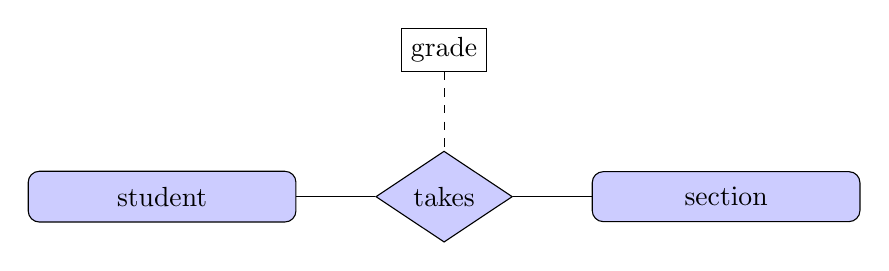
\begin{tikzpicture}
    \node (student) [draw, rounded corners,
    text centered, anchor=north, text=black, text width=3cm, fill=blue!20, inner sep=0.2cm] {student};

    \node (takes) [draw, diamond, aspect=1.5, fill=blue!20, right=of student] {takes};

    \node (section) [draw, rounded corners,
    text centered, anchor=north, text=black, text width=3cm, fill=blue!20, inner sep=0.2cm, right=of takes] {section};

    \draw (student) -- (takes);
    \draw (takes) -- (section);

    \node (grade) [draw, above=of takes]{grade};
    \draw [dashed] (grade) -- (takes);
\end{tikzpicture}

\alert{联系的描述性属性(descriptive attribute)}


\begin{tikzpicture}
    \node[fill=blue!30,blur shadow={shadow xshift=-0.5ex},
    text width=26em,anchor=south west,rounded corners]
    {E-R图可能很多页。这样一个实体可能在不同地方出现,只有第一次出现需要属性,其他地方仅出现实体名字就行。};
\end{tikzpicture}

\end{frame}

\begin{frame}
    \frametitle{2.3 属性}
\begin{exampleblock}{域(domain)}
    对于每个属性,都有一个可允许的取值集合,叫域(domain)。   
\end{exampleblock}
    
按不同标准,它可以分为:

\begin{itemize}
    \item \alert{简单}(simple)属性:不可再分;\alert{复合}(composite)属性:可以再划分为更小的部分(或其他属性)
    \item \alert{单值}(single-valued)属性;\alert{多值}(multi-valued)属性
\end{itemize}

\faIcon{lightbulb} 思考:有哪些复合属性和多值属性的例子?
\end{frame}

\begin{frame}[fragile]

    \begin{columns}
        \column{.4\textwidth}
        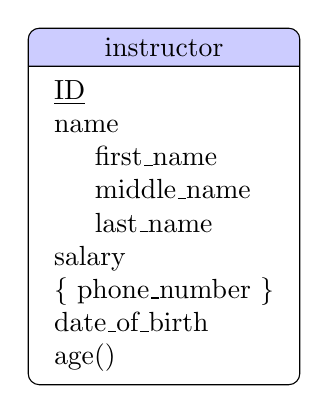
\begin{tikzpicture}[
            comment/.style={rectangle, draw=black, rounded corners,
            anchor=north, text=black, anchor=west}, every second node part/.style={fill=white}]
            \node (instructor) [comment, rectangle split, rectangle split parts=2, rectangle split part fill={blue!20,white}]
            {
                instructor
                \nodepart{second} 
                \begin{tabular}{l}
                    \underline{ID} \\
                    name \\ 
                    \hspace{4mm} first\_name \\
                    \hspace{4mm} middle\_name
                    \\
                    \hspace{4mm} last\_name \\
                    salary \\
                    \{ phone\_number \} \\
                    date\_of\_birth \\
                    age()\\
                \end{tabular}
            };
        \end{tikzpicture}
        \column{.6\textwidth}
        \faIcon{lightbulb} 王大锤同学在阅读课本的时候,发现有这么一句话:\alert{关系的每一个分量必须是一个不可分的数据项,也就是说,不允许表中还有表}(即属性的原子性)。那么为什么E-R图中可以出现复合属性和多值属性呢?
    \end{columns}

\end{frame}

\begin{frame}[fragile]

    \begin{columns}
        \column{.4\textwidth}
        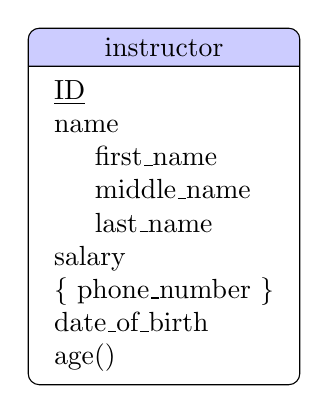
\begin{tikzpicture}[
            comment/.style={rectangle, draw=black, rounded corners,
            anchor=north, text=black, anchor=west}, every second node part/.style={fill=white}]
            \node (instructor) [comment, rectangle split, rectangle split parts=2, rectangle split part fill={blue!20,white}]
            {
                instructor
                \nodepart{second} 
                \begin{tabular}{l}
                    \underline{ID} \\
                    name \\ 
                    \hspace{4mm} first\_name \\
                    \hspace{4mm} middle\_name
                    \\
                    \hspace{4mm} last\_name \\
                    salary \\
                    \{ phone\_number \} \\
                    date\_of\_birth \\
                    age()\\
                \end{tabular}
            };
        \end{tikzpicture}
        \column{.6\textwidth}
        \faIcon{lightbulb} 如果实体集有了生日(birth)属性,那么是否需要年龄(age)属性? 对于之前的E-R图,教师实体集是否需要有「指导了多少名学生」这一属性?

        \pause

        \alert{派生(derived)属性}
    \end{columns}


\end{frame}

\begin{frame}
    \frametitle{2.4 映射基数}

\begin{exampleblock}{映射基数(mapping cardinality)}
    映射基数(mapping cardinality)表示一个实体通过一个联系集能关联的实体的个数。  
\end{exampleblock}

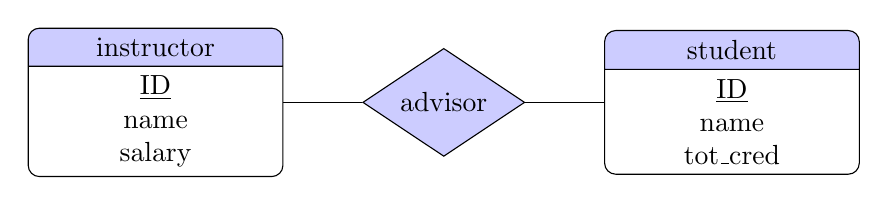
\begin{tikzpicture}[
    comment/.style={rectangle, draw=black, rounded corners,
    text centered, anchor=north, text=black, text width=3cm}, every second node part/.style={fill=white}]
    \node (instructor) [comment, rectangle split, rectangle split parts=2, rectangle split part fill={blue!20,white}]
    {
        instructor
        \nodepart{second} \underline{ID} \\ name \\ salary
    };

    \node (advisor) [fill=blue!20, draw, diamond, right=of instructor, aspect=1.5] {advisor}; 

    \node (student) [comment, rectangle split, rectangle split parts=2, rectangle split part fill={blue!20,white}, right=of advisor] {
        student
        \nodepart{second} \underline{ID} \\ name \\ tot\_cred 
    };

    \draw (instructor) -- (advisor);
    \draw (advisor) -- (student);
\end{tikzpicture}    

\alert{映射基数}是用来表示:一个教师能够指导多少学生?
一个学生能够被多少教师指导?
\end{frame}

\begin{frame}
    
    \begin{columns}
        \column{.6\textwidth}
        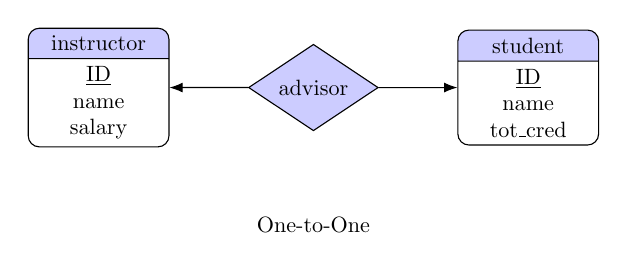
\begin{tikzpicture}[
            comment/.style={rectangle, draw=black, rounded corners,
            text centered, anchor=north, text=black, text width=2cm}, every second node part/.style={fill=white}, scale=0.8, every node/.style={scale=0.8}]
            \node (instructor) [comment, rectangle split, rectangle split parts=2, rectangle split part fill={blue!20,white},]
            {
                instructor
                \nodepart{second} \underline{ID} \\ name \\ salary
            };
        
            \node (advisor) [fill=blue!20, draw, diamond, right=of instructor, aspect=1.5] {advisor}; 
        
            \node (student) [comment, rectangle split, rectangle split parts=2, rectangle split part fill={blue!20,white}, right=of advisor] {
                student
                \nodepart{second} \underline{ID} \\ name \\ tot\_cred 
            };
        
            \draw [Latex-] (instructor) -- (advisor);
            \draw [-Latex] (advisor) -- (student);
            \node [below=of advisor] {One-to-One};
        \end{tikzpicture}      
        
        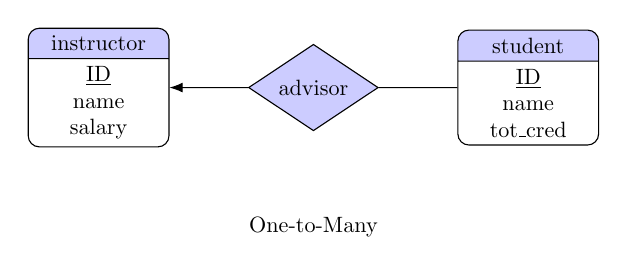
\begin{tikzpicture}[
            comment/.style={rectangle, draw=black, rounded corners,
            text centered, anchor=north, text=black, text width=2cm}, every second node part/.style={fill=white}, scale=0.8, every node/.style={scale=0.8}]
            \node (instructor) [comment, rectangle split, rectangle split parts=2, rectangle split part fill={blue!20,white}]
            {
                instructor
                \nodepart{second} \underline{ID} \\ name \\ salary
            };
        
            \node (advisor) [fill=blue!20, draw, diamond, right=of instructor, aspect=1.5] {advisor}; 
        
            \node (student) [comment, rectangle split, rectangle split parts=2, rectangle split part fill={blue!20,white}, right=of advisor] {
                student
                \nodepart{second} \underline{ID} \\ name \\ tot\_cred 
            };
        
            \draw [Latex-] (instructor) -- (advisor);
            \draw (advisor) -- (student);
            \node [below=of advisor] {One-to-Many};
        \end{tikzpicture}
        \column{.4\textwidth}
        \faIcon{lightbulb} 猜测Many-to-Many和Many-to-One应该如何表示?
    \end{columns}
\end{frame}

\begin{frame}[fragile]
    \frametitle{2.5 基数约束}

约束可以使用一对数\alert{min..max}表示。

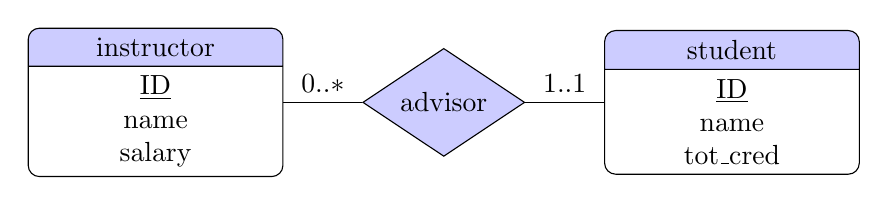
\begin{tikzpicture}[
    comment/.style={rectangle, draw=black, rounded corners,
    text centered, anchor=north, text=black, text width=3cm}, every second node part/.style={fill=white}]
    \node (instructor) [comment, rectangle split, rectangle split parts=2, rectangle split part fill={blue!20,white}]
    {
        instructor
        \nodepart{second} \underline{ID} \\ name \\ salary
    };

    \node (advisor) [fill=blue!20, draw, diamond, right=of instructor, aspect=1.5] {advisor}; 

    \node (student) [comment, rectangle split, rectangle split parts=2, rectangle split part fill={blue!20,white}, right=of advisor] {
        student
        \nodepart{second} \underline{ID} \\ name \\ tot\_cred 
    };

    \draw (instructor) -- node[above] {0..$\ast$} ++ (advisor);
    \draw (advisor) -- node [above] {1..1} ++ (student);
\end{tikzpicture}   

按教材的规定,每个教师都恰好有一个学生,且每个学生被0到多个教师指导;但《Database System Concepts》一书中恰好相反。
\end{frame}

\begin{frame}
实体的「全」参与,使用\alert{两条线}表示:
    
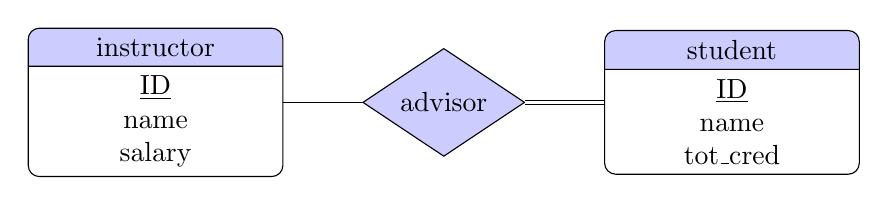
\begin{tikzpicture}[
    comment/.style={rectangle, draw=black, rounded corners,
    text centered, anchor=north, text=black, text width=3cm}, every second node part/.style={fill=white}]
    \node (instructor) [comment, rectangle split, rectangle split parts=2, rectangle split part fill={blue!20,white}]
    {
        instructor
        \nodepart{second} \underline{ID} \\ name \\ salary
    };

    \node (advisor) [fill=blue!20, draw, diamond, right=of instructor, aspect=1.5] {advisor}; 

    \node (student) [comment, rectangle split, rectangle split parts=2, rectangle split part fill={blue!20,white}, right=of advisor] {
        student
        \nodepart{second} \underline{ID} \\ name \\ tot\_cred 
    };

    \draw (instructor) -- (advisor);
    \draw [double, double distance = 1pt] (advisor) -- (student);
\end{tikzpicture}   

上面的E-R图表示每个学生都有导师。
\end{frame}

\begin{frame}
    \frametitle{2.6 E-R软件}
在线工具:

\begin{itemize}
    \item LucidChart
    \item Draw.io(推荐)
\end{itemize}
    
专业工具:

\begin{itemize}
    \item IBM Rational Rose Modeler
    \item Microsoft Visio
    \item ERWin
    \item SmartDraw    
\end{itemize}

\end{frame}

\begin{frame}

\begin{columns}
    \column{.3\textwidth}
    DataGrip的可视化:点击右边栏 tables,右键选择 Diagrams,点击 Show Visualization。
    \column{.7\textwidth}
    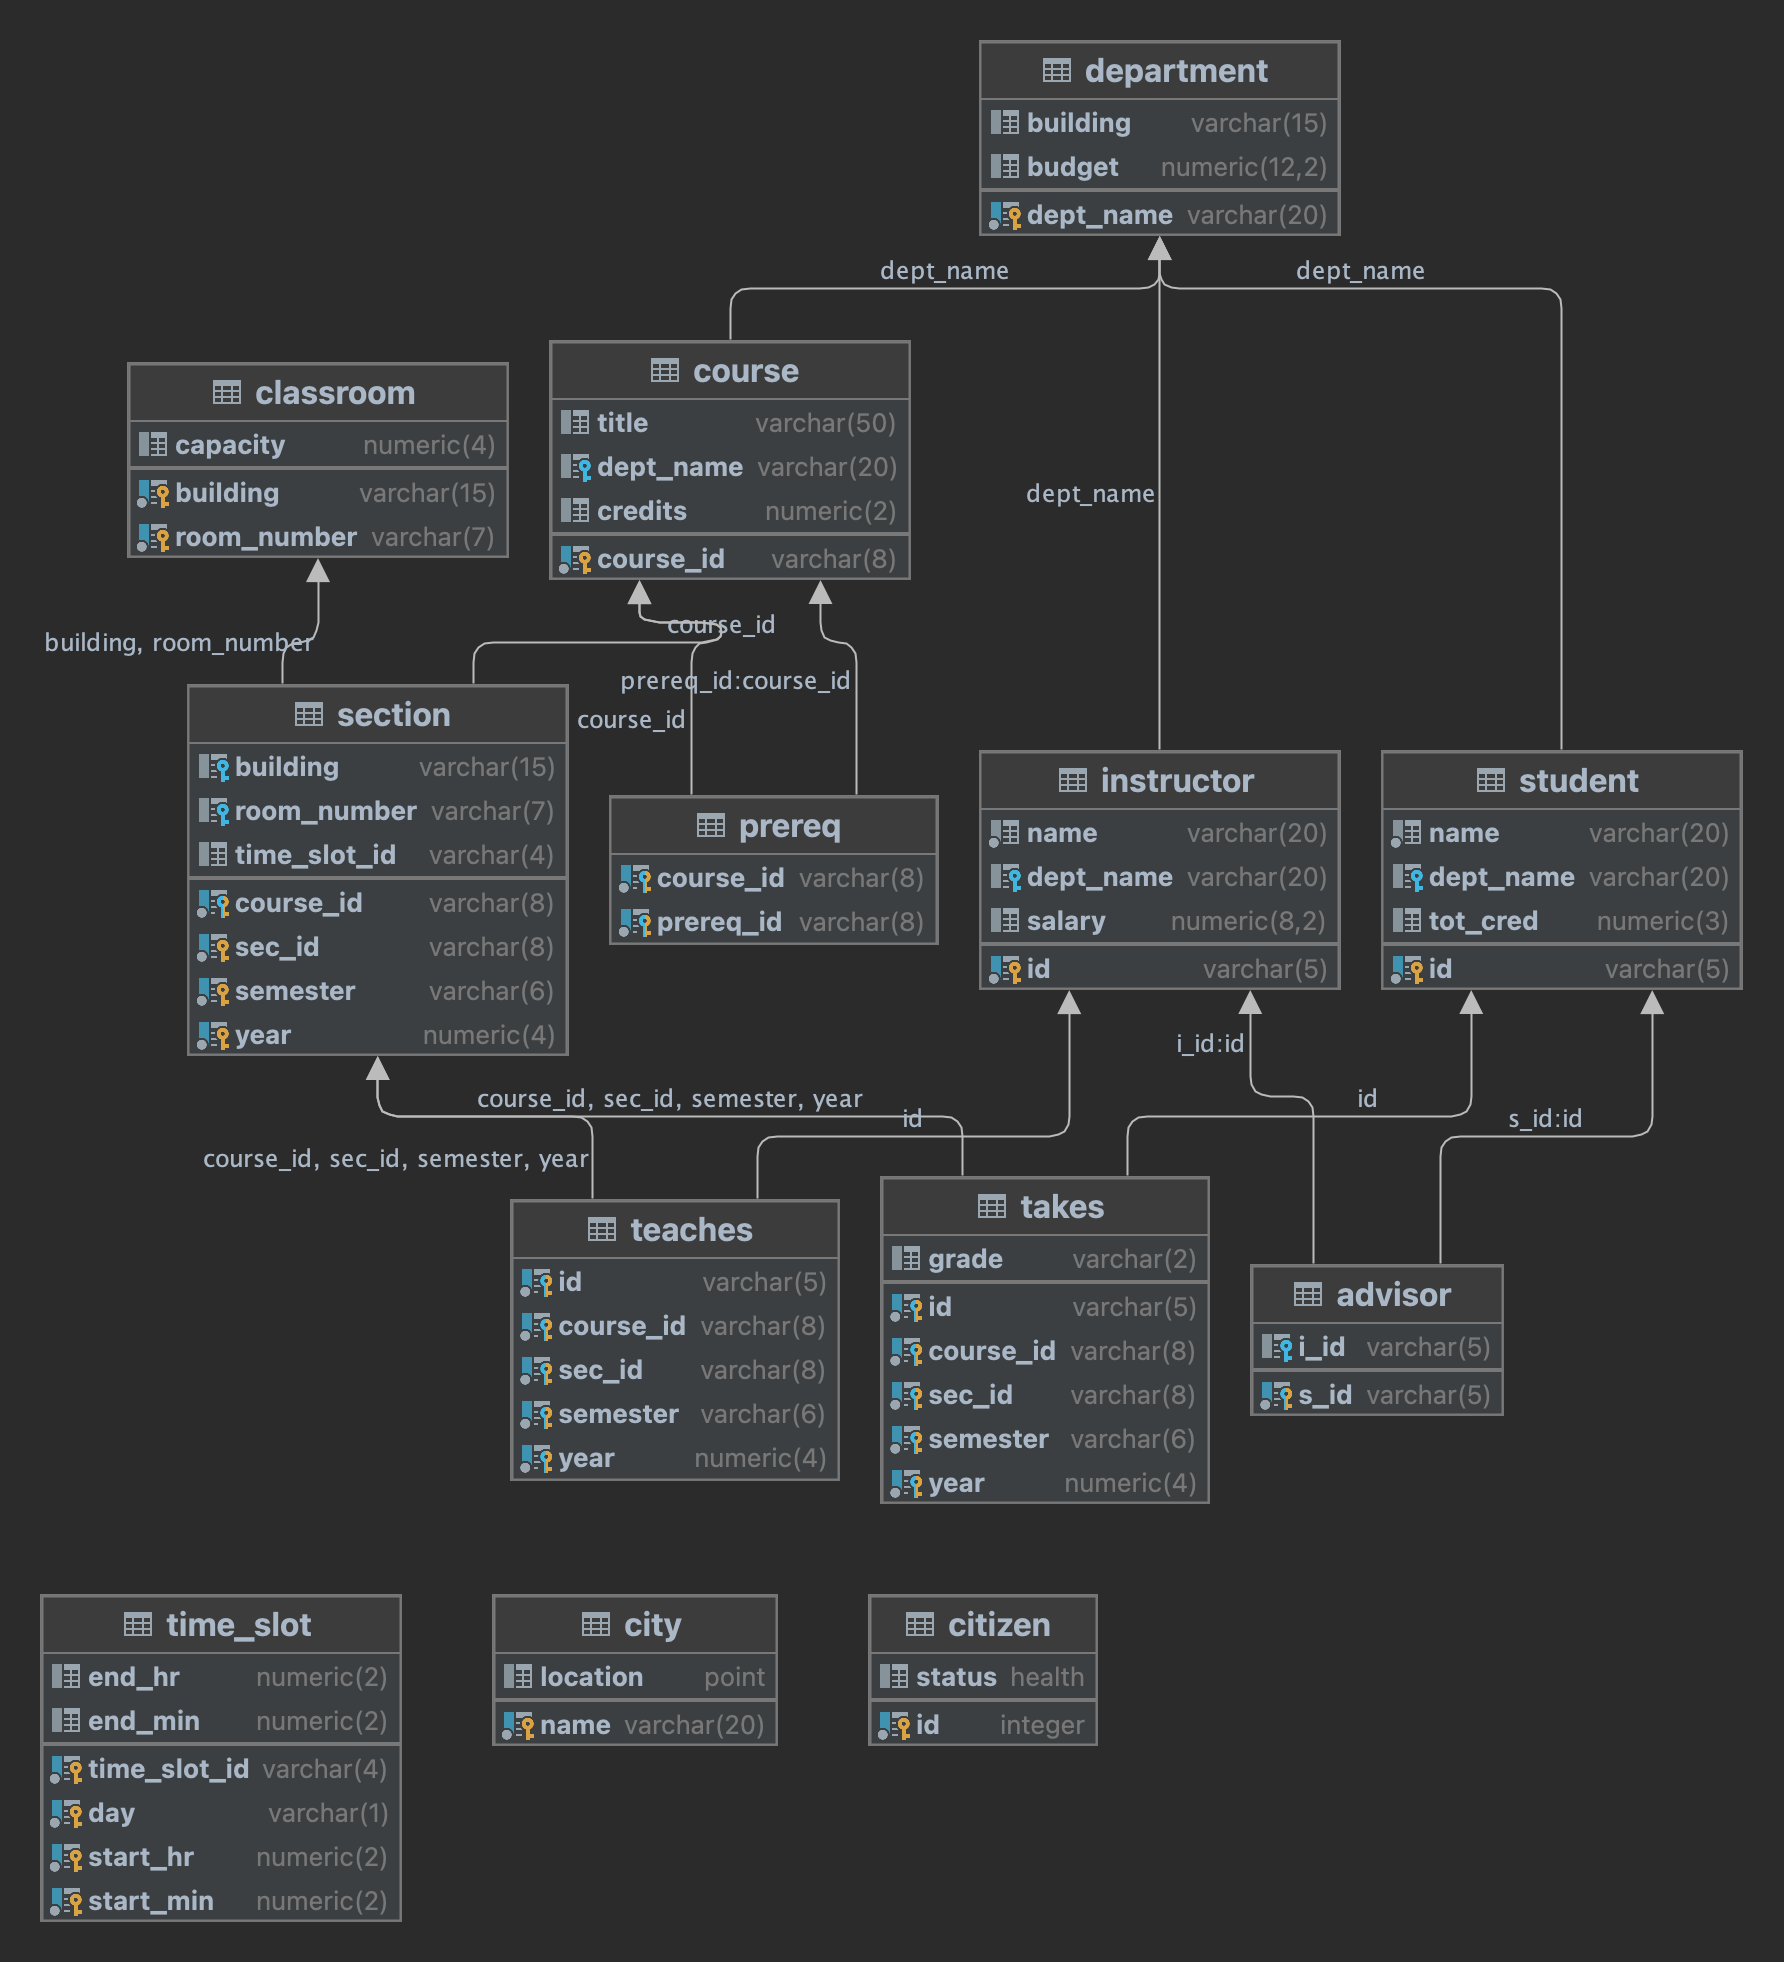
\includegraphics[width=.9\textwidth]{week10/uml}
\end{columns}

\end{frame}

\begin{frame}
    \section{\textcolor{darkmidnightblue}{3. 主码}}
    与关系类似,E-R模型中也有主码的概念,用来唯一标识一个实体或联系。
\end{frame}

\begin{frame}
    \frametitle{3.1 实体集的主码}
之前学习的“关系模式”的码(包括候选码、主码)的概念可以直接用于实体集。

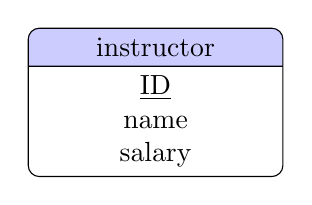
\begin{tikzpicture}[
    comment/.style={rectangle, draw=black, rounded corners,
    text centered, anchor=north, text=black, text width=3cm}, every second node part/.style={fill=white}]
    \node [comment, rectangle split, rectangle split parts=2, rectangle split part fill={blue!20,white}]
    {
        instructor
        \nodepart{second} \underline{ID} \\ name \\ salary
    };
\end{tikzpicture}

\end{frame}

\begin{frame}[fragile]
    \frametitle{3.2 联系集的主码}
\begin{block}{联系集的超码}
$PK(E_1) \cup PK(E_2) \cup \dots \cup PK(E_n)$构成联系集的超码。    
\end{block}
    
\alert{情况一:One-to-Many或Many-to-One}

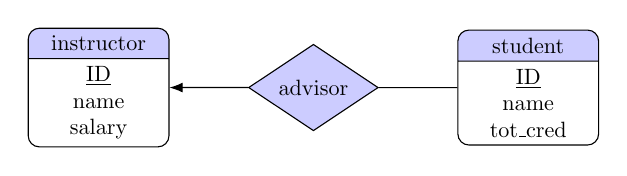
\begin{tikzpicture}[
    comment/.style={rectangle, draw=black, rounded corners,
    text centered, anchor=north, text=black, text width=2cm}, every second node part/.style={fill=white}, scale=0.8, every node/.style={scale=0.8}]
    \node (instructor) [comment, rectangle split, rectangle split parts=2, rectangle split part fill={blue!20,white},]
    {
        instructor
        \nodepart{second} \underline{ID} \\ name \\ salary
    };

    \node (advisor) [fill=blue!20, draw, diamond, right=of instructor, aspect=1.5] {advisor}; 

    \node (student) [comment, rectangle split, rectangle split parts=2, rectangle split part fill={blue!20,white}, right=of advisor] {
        student
        \nodepart{second} \underline{ID} \\ name \\ tot\_cred 
    };

    \draw [Latex-] (instructor) -- (advisor);
    \draw (advisor) -- (student);
\end{tikzpicture}   

\faIcon{lightbulb} Many还是One一侧实体集的主码可以构成联系集的主码?
\end{frame}

\begin{frame}
\faIcon{lightbulb} 思考:对于One-to-One和Many-to-Many应该如何选择主码?

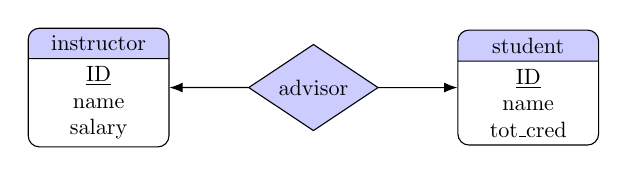
\begin{tikzpicture}[
    comment/.style={rectangle, draw=black, rounded corners,
    text centered, anchor=north, text=black, text width=2cm}, every second node part/.style={fill=white}, scale=0.8, every node/.style={scale=0.8}]
    \node (instructor) [comment, rectangle split, rectangle split parts=2, rectangle split part fill={blue!20,white},]
    {
        instructor
        \nodepart{second} \underline{ID} \\ name \\ salary
    };

    \node (advisor) [fill=blue!20, draw, diamond, right=of instructor, aspect=1.5] {advisor}; 

    \node (student) [comment, rectangle split, rectangle split parts=2, rectangle split part fill={blue!20,white}, right=of advisor] {
        student
        \nodepart{second} \underline{ID} \\ name \\ tot\_cred 
    };

    \draw [Latex-] (instructor) -- (advisor);
    \draw [-Latex] (advisor) -- (student);
\end{tikzpicture}   

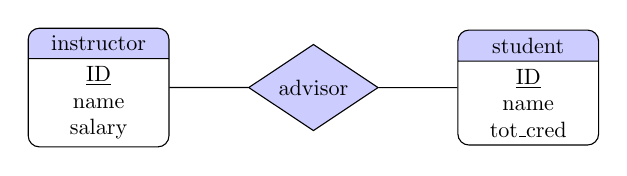
\begin{tikzpicture}[
    comment/.style={rectangle, draw=black, rounded corners,
    text centered, anchor=north, text=black, text width=2cm}, every second node part/.style={fill=white}, scale=0.8, every node/.style={scale=0.8}]
    \node (instructor) [comment, rectangle split, rectangle split parts=2, rectangle split part fill={blue!20,white},]
    {
        instructor
        \nodepart{second} \underline{ID} \\ name \\ salary
    };

    \node (advisor) [fill=blue!20, draw, diamond, right=of instructor, aspect=1.5] {advisor}; 

    \node (student) [comment, rectangle split, rectangle split parts=2, rectangle split part fill={blue!20,white}, right=of advisor] {
        student
        \nodepart{second} \underline{ID} \\ name \\ tot\_cred 
    };

    \draw (instructor) -- (advisor);
    \draw (advisor) -- (student);
\end{tikzpicture}  

\end{frame}


\begin{frame}
    \frametitle{3.3 弱实体集}
考虑\texttt{section},它需要依赖另外一个实体而存在,我们把这样的实体称为\alert{弱实体集}(weak entity set)。
    
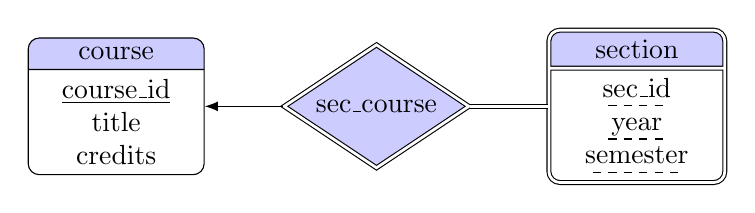
\begin{tikzpicture}[
    comment/.style={rectangle, draw=black, rounded corners,
    text centered, anchor=north, text=black, text width=2cm}, every second node part/.style={fill=white},]
    \node (course) [comment, rectangle split, rectangle split parts=2, rectangle split part fill={blue!20,white},]
    {
        course
        \nodepart{second} \underline{course\_id} \\ title \\ credits
    };

    \node (seccourse) [fill=blue!20, draw, diamond, right=of course, aspect=1.5, double, double distance=1pt] {sec\_course}; 

    \node (section) [comment, rectangle split, rectangle split parts=2, rectangle split part fill={blue!20,white}, right=of seccourse, double, double distance=1pt] {
        section
        \nodepart{second} \dashuline{sec\_id} \\ \dashuline{year} \\ \dashuline{semester} 
    };

    \draw [Latex-] (course) -- (seccourse);
    \draw [double, double distance=1pt] (seccourse) -- (section);
\end{tikzpicture}  

\textbf{弱实体集的主码由标识实体集(identifying entity set)的主码加上该弱实体集的分辨符(discriminator)构成。}
\end{frame}

\begin{frame}
    \frametitle{3.4 去除冗余属性}
在使用E-R模型的时候,\textbf{要确保实体间不存在冗余属性}(\alert{a good entity-relationship design does not contain redundant attributes})。

比如考虑:\texttt{instructor(ID, name, dept\_name, salary)}和\texttt{department(dept\_name, building, budget)}。

\end{frame}

\begin{frame}[fragile]

    \begin{tikzpicture}[
        comment/.style={rectangle, draw=black, rounded corners,
        text centered, anchor=north, text=black, text width=2.5cm}, every second node part/.style={fill=white},  scale=0.6, every node/.style={scale=0.6}]
        \node (department) [comment, rectangle split, rectangle split parts=2, rectangle split part fill={blue!20,white},]
        {
            department
            \nodepart{second} \underline{dept\_name} \\ building \\ budget
        };
        \node (studept) [diamond, draw, below right=of department, aspect=1.6, fill=blue!20] {stud\_dept};

        \node (student) [comment, rectangle split, rectangle split parts=2, rectangle split part fill={blue!20,white}, below right=of studept]
        {
            student
            \nodepart{second} \underline{ID} \\ name \\ tot\_cred
        };

        \draw [Latex-] (department) -- (studept);
        \draw [double, double distance=1.2pt] (studept) -- (student);

        \node (instdept) [diamond, draw, below left=of department, aspect=1.6, fill=blue!20] {inst\_dept};

        \node (instructor) [comment, rectangle split, rectangle split parts=2, rectangle split part fill={blue!20,white}, below left=of instdept]
        {
            instructor
            \nodepart{second} \underline{ID} \\ name \\ salary
        };

        \draw [Latex-] (department) -- (instdept);
        \draw [double, double distance=1.2pt] (instdept) -- (instructor);

        \node (advisor) [diamond, draw, below=of department, aspect=1.6, fill=blue!20, ] {advisor};

        \draw [Latex-] (instructor) -- (advisor);
        \draw (advisor) -- (student);

        \node (teaches) [diamond, draw, right=of instructor, aspect=1.6, fill=blue!20,] {teaches};
        
        \node (takes) [diamond, draw, left=of student, aspect=1.6, fill=blue!20,] {takes};

        \node (grade) [left=of takes, draw] {grade};
        \draw [dashed] (takes) -- (grade);

        \node (section) [comment, rectangle split, rectangle split parts=2, rectangle split part fill={blue!20,white}, below left=of takes, double, double distance=1pt] {
            section
            \nodepart{second} \dashuline{sec\_id} \\ \dashuline{year} \\ \dashuline{semester} 
        };

        \draw (instructor) -- (teaches);
        \draw [double, double distance=1.2pt] (teaches) -- (section);

        \draw (student) -- (takes);
        \draw (takes) -- (section);

        \node (coursedept) [diamond, draw, left=of department, xshift=-7cm, aspect=1.6, fill=blue!20,] {course\_dept};

        \draw [-Latex] (coursedept) -- (department);

        \node (course) [comment, rectangle split, rectangle split parts=2, rectangle split part fill={blue!20,white}, below =of coursedept, yshift=-3cm,]
        {
            course
            \nodepart{second} \underline{ID} \\ name \\ salary
        };

        \draw [double, double distance=1.2pt] (coursedept) -- (course);

        \node (seccourse) [fill=blue!20, draw, diamond, below right=of course, aspect=1.5, double, double distance=1pt] {sec\_course}; 

        \draw [Latex-] (course) -- (seccourse);

        \draw [double, double distance=1.2pt] (seccourse) -- (section);
        
        \node (prereq) [diamond, draw, below=of course, aspect=1.6, fill=blue!20,] {prereq};

        \draw (course) -- node [right] {prereq\_id} ++ (prereq);
        
        \draw (prereq.west) -- node [below] {course\_id} ++(-1,0) |- ($ (course.west) + (-.6, 0)$) -- (course.west);

        \node [red, right=of section, align=left] {忽略了time\_slot和 \\classroom两个实体。}; 

    \end{tikzpicture}


\end{frame}

\begin{frame}
    \frametitle{练习}
    \faIcon{basketball-ball} 考虑NBA比赛中「记录球员参加比赛的得分」这一需求,绘制E-R图。



\includegraphics[width=.99\textwidth]{week10/nba}
\end{frame}

\begin{frame}[fragile]

    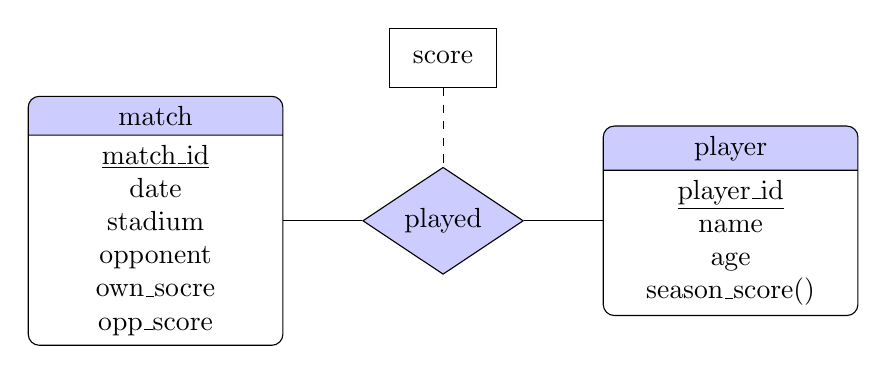
\begin{tikzpicture}[
        comment/.style={rectangle, draw=black, rounded corners,
        text centered, anchor=north, text=black, text width=3cm}, every second node part/.style={fill=white},]
        \node (match) [comment, rectangle split, rectangle split parts=2, rectangle split part fill={blue!20,white},]
        {
            match
            \nodepart{second} \underline{match\_id} \\ date \\ stadium \\ opponent \\ own\_socre \\ opp\_score
        };
    
        \node (played) [fill=blue!20, draw, diamond, right=of match, aspect=1.5,] {played}; 
    
        \node (player) [comment, rectangle split, rectangle split parts=2, rectangle split part fill={blue!20,white}, right=of played] {
            player
            \nodepart{second} \underline{player\_id} \\ name \\ age \\ season\_score()
        };
    
        \draw (match) -- (played);
        \draw (played) -- (player);

        \node (score) [draw, above=of played, inner sep=.3cm] {score};
        \draw [dashed] (score) -- (played);
    \end{tikzpicture}  

\end{frame}

\begin{frame}
    \section{\textcolor{darkmidnightblue}{4. E-R图转化为关系模式}}
    \begin{tikzpicture}[>=stealth,
        node distance = 3mm and 3mm,
          start chain = A going below right,
    every node/.style = {draw, text width=24mm, minimum height=12mm, align=center,
                         inner sep=1mm, fill=white, drop shadow={fill=black},  on chain=A},
                            ]
    \node (nreq) {需求分析}; % A-1
    \node {概念设计};
    \node {逻辑设计};
    \node {物理设计};
    %
    \foreach \i [count=\j] in {2,...,4}
    {
    %   \draw[->, thick] (A-\i) -| (A-\j);
      \draw[->, thick] (A-\j) -| (A-\i);
    }
    \end{tikzpicture}
\end{frame}

\begin{frame}
    \frametitle{4.1 具有简单属性的强实体集}

    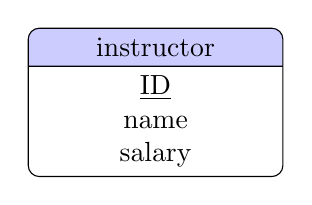
\begin{tikzpicture}[
        comment/.style={rectangle, draw=black, rounded corners,
        text centered, anchor=north, text=black, text width=3cm}, every second node part/.style={fill=white}]
        \node [comment, rectangle split, rectangle split parts=2, rectangle split part fill={blue!20,white}]
        {
            instructor
            \nodepart{second} \underline{ID} \\ name \\ salary
        };
    \end{tikzpicture}

    \texttt{instructor(\underline{ID}, name, salary)}

\end{frame}

\begin{frame}[fragile]
    \frametitle{4.2 具有复杂属性的强实体集}
    \begin{columns}
        \column{.4\textwidth}
        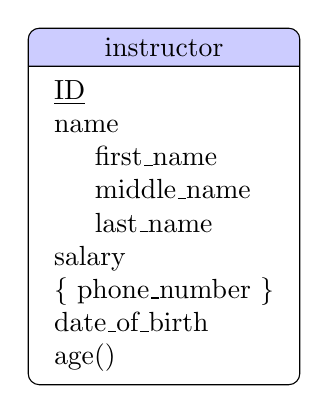
\begin{tikzpicture}[
            comment/.style={rectangle, draw=black, rounded corners,
            anchor=north, text=black, anchor=west}, every second node part/.style={fill=white}]
            \node (instructor) [comment, rectangle split, rectangle split parts=2, rectangle split part fill={blue!20,white}]
            {
                instructor
                \nodepart{second} 
                \begin{tabular}{l}
                    \underline{ID} \\
                    name \\ 
                    \hspace{4mm} first\_name \\
                    \hspace{4mm} middle\_name
                    \\
                    \hspace{4mm} last\_name \\
                    salary \\
                    \{ phone\_number \} \\
                    date\_of\_birth \\
                    age()\\
                \end{tabular}
            };
        \end{tikzpicture}
        \column{.6\textwidth}
        \begin{itemize}
            \item \texttt{instructor(\underline{ID}, first\_name, middle\_name, last\_name, salary, date\_of\_birth)}
            \item \texttt{instructor\_phone(ID, phone\_number)}
        \end{itemize}

        \faIcon{lightbulb} 思考:关系\texttt{instructor\_phone}的主码是什么?
    \end{columns}

\end{frame}
\begin{frame}
    \frametitle{4.3 弱实体集}
    设A是具有属性$a_1,a_2,\dots, a_m$的弱实体集,设B是A所依赖的强实体集,B的主码包括属性$b_1,b_2,\dots, b_n$。那么A对应的关系模式包括属性:

    \[\{a_1,a_2, \dots, a_m\} \cup \{b_1,b_2,\dots, b_n \}\]


    \begin{columns}
        \column{.6\textwidth}
        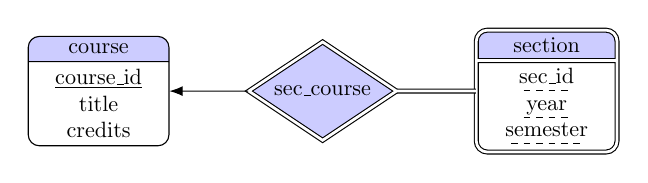
\begin{tikzpicture}[
            comment/.style={rectangle, draw=black, rounded corners,
            text centered, anchor=north, text=black, text width=2cm}, every second node part/.style={fill=white},scale=0.8, every node/.style={scale=0.8}]
            \node (course) [comment, rectangle split, rectangle split parts=2, rectangle split part fill={blue!20,white},]
            {
                course
                \nodepart{second} \underline{course\_id} \\ title \\ credits
            };
        
            \node (seccourse) [fill=blue!20, draw, diamond, right=of course, aspect=1.5, double, double distance=1pt] {sec\_course}; 
        
            \node (section) [comment, rectangle split, rectangle split parts=2, rectangle split part fill={blue!20,white}, right=of seccourse, double, double distance=1pt] {
                section
                \nodepart{second} \dashuline{sec\_id} \\ \dashuline{year} \\ \dashuline{semester} 
            };
        
            \draw [Latex-] (course) -- (seccourse);
            \draw [double, double distance=1pt] (seccourse) -- (section);
        \end{tikzpicture}  
        \column{.4\textwidth}   
        \texttt{section(\underline{course\_id}, \underline{sec\_id}, \underline{year}, \underline{semester})}
    \end{columns}
\end{frame}


\begin{frame}
    \frametitle{4.4 联系集}
    设R是联系集,设$a_1, a_2, \dots, a_m$是所有参与R的实体集的主码的并集,设R的描述性属性(如果有)为$b_1, b_2, \dots, b_n$,那么R对应的关系模式包括属性:

    \[\{a_1, a_2, \dots, a_m\} \cup \{ b_1, b_2, \dots, b_n \}\]

    \begin{columns}
        \column{.6\textwidth}
        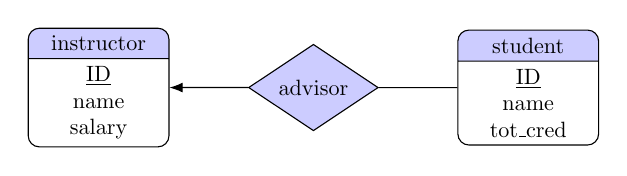
\begin{tikzpicture}[
            comment/.style={rectangle, draw=black, rounded corners,
            text centered, anchor=north, text=black, text width=2cm}, every second node part/.style={fill=white}, scale=0.8, every node/.style={scale=0.8}]
            \node (instructor) [comment, rectangle split, rectangle split parts=2, rectangle split part fill={blue!20,white},]
            {
                instructor
                \nodepart{second} \underline{ID} \\ name \\ salary
            };
        
            \node (advisor) [fill=blue!20, draw, diamond, right=of instructor, aspect=1.5] {advisor}; 
        
            \node (student) [comment, rectangle split, rectangle split parts=2, rectangle split part fill={blue!20,white}, right=of advisor] {
                student
                \nodepart{second} \underline{ID} \\ name \\ tot\_cred 
            };
        
            \draw [Latex-] (instructor) -- (advisor);
            \draw (advisor) -- (student);
        \end{tikzpicture}   
        \column{.4\textwidth}
        \faIcon{comment-dots} 回忆一下二元联系中R的主码如何选择?
    \end{columns}

\end{frame}

\begin{frame}
通过上面的方法,可以得到所有\textbf{联系集}的关系模式:
\begin{itemize}
    \item \texttt{teaches(\underline{ID}, \underline{course\_id}, \underline{sec\_id}, semeter, year)}
    \item \texttt{takes(\underline{ID}, \underline{course\_id}, \underline{sec\_id}, \underline{semester}, \underline{year}, grade)}
    \item \texttt{advisor(\underline{s\_ID}, i\_ID)}
    \item \dots
    \item \texttt{inst\_dept(\underline{ID}, dept\_name)}
    \item \texttt{course\_dept(\underline{course\_id}, dept\_name)}
\end{itemize}

注意到很多关系模式在大学数据库中并没有出现,所以一个自然而然的问题是:\alert{到底哪些模式应该保留,而哪些模式应该删除呢?}
\end{frame}

\begin{frame}
    \frametitle{4.5 模式的冗余}

\begin{exampleblock}{冗余}
    连接弱实体集与其依赖的强实体集的联系集的模式是冗余的。
\end{exampleblock}

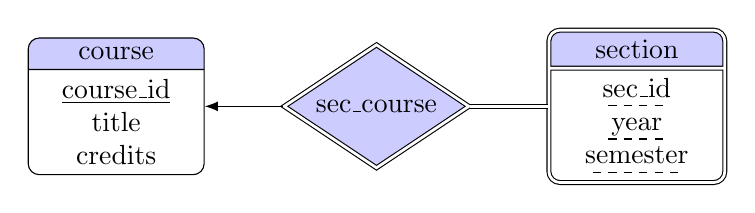
\begin{tikzpicture}[
    comment/.style={rectangle, draw=black, rounded corners,
    text centered, anchor=north, text=black, text width=2cm}, every second node part/.style={fill=white},]
    \node (course) [comment, rectangle split, rectangle split parts=2, rectangle split part fill={blue!20,white},]
    {
        course
        \nodepart{second} \underline{course\_id} \\ title \\ credits
    };

    \node (seccourse) [fill=blue!20, draw, diamond, right=of course, aspect=1.5, double, double distance=1pt] {sec\_course}; 

    \node (section) [comment, rectangle split, rectangle split parts=2, rectangle split part fill={blue!20,white}, right=of seccourse, double, double distance=1pt] {
        section
        \nodepart{second} \dashuline{sec\_id} \\ \dashuline{year} \\ \dashuline{semester} 
    };

    \draw [Latex-] (course) -- (seccourse);
    \draw [double, double distance=1pt] (seccourse) -- (section);
\end{tikzpicture}  

\faIcon{edit} 提示:比较\texttt{sec\_course}和\texttt{section}的关系模式的异同。
\end{frame}

\begin{frame}
    \frametitle{4.6 模式的合并}
Many-to-One的联系可以让联系和Many一侧的实体合并。
    
\begin{tikzpicture}[
    comment/.style={rectangle, draw=black, rounded corners,
    text centered, anchor=north, text=black, text width=3cm}, every second node part/.style={fill=white},]
    \node (instructor) [comment, rectangle split, rectangle split parts=2, rectangle split part fill={blue!20,white},]
    {
        instructor
        \nodepart{second} \underline{ID} \\ name \\ salary
    };

    \node (insdept) [fill=blue!20, draw, diamond, right=of instructor, aspect=1.5] {ins\_dept}; 

    \node (department) [comment, rectangle split, rectangle split parts=2, rectangle split part fill={blue!20,white}, right=of insdept] {
        department
        \nodepart{second} \underline{dept\_name} \\ building \\ budget 
    };

    \draw [double, double distance=1.2pt] (instructor) -- (insdept);
    \draw [-Latex] (insdept) -- (department);

    \node [red, below right=of instructor] (merge) {合并(取并集)};

    \draw [draw, red] (instructor) -- (merge);
    \draw [draw, red] (insdept) -- (merge);
\end{tikzpicture}   

\end{frame}

\begin{frame}
    \frametitle{思考}
One-to-One的联系能否合并?如果能的话,如何合并?
    
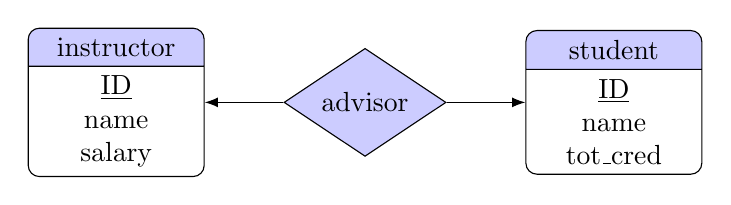
\begin{tikzpicture}[
    comment/.style={rectangle, draw=black, rounded corners,
    text centered, anchor=north, text=black, text width=2cm}, every second node part/.style={fill=white},]
    \node (instructor) [comment, rectangle split, rectangle split parts=2, rectangle split part fill={blue!20,white},]
    {
        instructor
        \nodepart{second} \underline{ID} \\ name \\ salary
    };

    \node (advisor) [fill=blue!20, draw, diamond, right=of instructor, aspect=1.5] {advisor}; 

    \node (student) [comment, rectangle split, rectangle split parts=2, rectangle split part fill={blue!20,white}, right=of advisor] {
        student
        \nodepart{second} \underline{ID} \\ name \\ tot\_cred 
    };

    \draw [Latex-] (instructor) -- (advisor);
    \draw [-Latex] (advisor) -- (student);
\end{tikzpicture}   

\end{frame}

\begin{frame}
    \frametitle{练习}
根据下面的E-R图写出关系模式。

    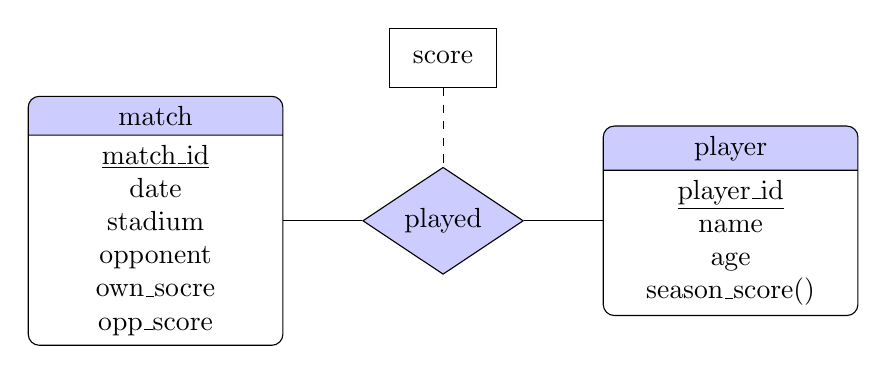
\begin{tikzpicture}[
        comment/.style={rectangle, draw=black, rounded corners,
        text centered, anchor=north, text=black, text width=3cm}, every second node part/.style={fill=white},]
        \node (match) [comment, rectangle split, rectangle split parts=2, rectangle split part fill={blue!20,white},]
        {
            match
            \nodepart{second} \underline{match\_id} \\ date \\ stadium \\ opponent \\ own\_socre \\ opp\_score
        };
    
        \node (played) [fill=blue!20, draw, diamond, right=of match, aspect=1.5,] {played}; 
    
        \node (player) [comment, rectangle split, rectangle split parts=2, rectangle split part fill={blue!20,white}, right=of played] {
            player
            \nodepart{second} \underline{player\_id} \\ name \\ age \\ season\_score()
        };
    
        \draw (match) -- (played);
        \draw (played) -- (player);

        \node (score) [draw, above=of played, inner sep=.3cm] {score};
        \draw [dashed] (score) -- (played);
    \end{tikzpicture}  

\end{frame}


\begin{frame}
    \section{\textcolor{darkmidnightblue}{小结}}
    \begin{itemize}
        \item E-R模型
        \item 将E-R图转化成关系模式
        \item E-R模型的替代品(如UML图)
    \end{itemize}
\end{frame}
\end{document}
